\documentclass[11pt,a4paper]{article}

% ---------- FONT & LANGUAGE ----------
\usepackage[T1]{fontenc}
\usepackage[utf8]{inputenc}
\usepackage[english]{babel}
\usepackage{amsmath,amsfonts,amssymb}
\let\Bbbk\relax
\usepackage{newtxtext,newtxmath} % Times New Roman equivalent
\usepackage[pdftex]{graphicx} 
\usepackage{fancyhdr}
\usepackage{svg}

\usepackage{afterpage}
\usepackage{setspace}
\usepackage{bibspacing}
\singlespacing


% ---------- PAGE LAYOUT ----------
\usepackage[a4paper,margin=2.5cm,
  headheight=1.8cm,headsep=0.5cm]{geometry}
\setlength{\parindent}{0pt}
\setlength{\parskip}{6pt}


% ---------- SECTION TITLES ----------
\usepackage{titlesec}
\titleformat{\section}
  {\normalfont\bfseries\fontsize{12pt}{13.8pt}\selectfont}
  {\thesection.}{0.5em}{}
\titlespacing*{\section}{0pt}{12pt plus 2pt}{6pt}
% \titlespacing{command}{left spacing}{before spacing}{after spacing}[right]
% Spacing: how to read {12pt plus 4pt minus 2pt}
% 12pt is what we would like the spacing to be.
% plus 4pt means that TeX can stretch it by at most 4pt.
% minus 2pt means that TeX can shrink it by at most 2pt.
% This is one example of the concept of, 'glue', in TeX.

\titleformat{\subsection}
  {\normalfont\bfseries\fontsize{11pt}{12pt}\selectfont}
  {\thesubsection\;}{0em}{}
\titlespacing*{\subsection}{0pt}{6pt plus 1pt}{3pt}


%% ---------- ICCFD13 HEADER ----------

\pagestyle{fancy}
\fancyhf{} % clear header and footer
\fancyhead[L]{\raggedright \small \bf Thirteenth International Conference on       
Computational Fluid Dynamics (ICCFD13)\\
Milan, Italy, July 06-10, 2026\\
}
\fancyhead[R]{\thepage\\}

\renewcommand{\headrulewidth}{0pt}


% ---- Custom first-page style ----
\fancypagestyle{firstpage}{
\fancyhf{} % clear all header and footer fields
\fancyhead[L]{
\includegraphics[height=1.2cm]{iccfd13_banner}} % Logo on the left header


\renewcommand{\headrulewidth}{0pt}
}

\setlength{\headsep}{0cm} % Adjust the space after the header

%% TITLE
\makeatletter
\def\@maketitle{%
  \thispagestyle{firstpage}% apply the custom header automatically
  \begin{center}
    \vspace*{0cm}
    {\LARGE\bfseries \@title \par}
    \vspace{6pt}
    {\large \@author \par}
    \vspace{0.5em}
  \end{center}
}
\makeatother



% Figure and equation label and reference:
\newcommand{\equa}[1]{(\ref{eq:#1})}
\newcommand{\laeq}[1]{\label{eq:#1}}
\newcommand{\figu}[1]{\ref{fig:#1}}
\newcommand{\lafi}[1]{\label{fig:#1}}

\title{
AW-FNO: An Adaptive approach for Fluid flow Super-resolution via Gated Wavelet-Fourier Learning
}

\author{Mamta Saini$^{**}$, Parikshit Mahajan$^{*}$, Gazania Marine Jyrwa$^{**}$, Diya Nagchaudhury$^{*}$, and Sashikumaar Ganesan$^{*,**}$\\
Corresponding author: sashi@iisc.ac.in \\
$^{*}$ Indian Institute of Science, Bengaluru, India.\\
$^{**}$ ZenteiQ Aitech Innovations Pvt. Ltd.
}
\date{}



% ---------- DOCUMENT ----------
\begin{document}

\maketitle
\thispagestyle{firstpage}



%%%% KEYWORDS
%\vskip0.5cm
\centerline{
\begin{minipage}[t]{150mm}
{\it Keywords:} Numerical algorithms, Scientific machine learning, Neural operators, Turbulent flows. \\
\end{minipage}
}




\section{Introduction}

% The numerical simulation of fluid flows, particularly at high Reynolds numbers, remains a significant challenge in fluid dynamics. The generation of high-fidelity (HF) data using Direct Numerical Simulation (DNS) is computationally intensive and demands substantial computational resources. Consequently, super-resolution (SR), defined as the reconstruction of high-resolution flow fields from low-resolution (LR) data, has emerged as an important area of research.

% In turbulent flows, energy is transferred from large-scale eddies to the smaller scales. Standard CNNs are limited by local receptive fields. Recently, Neural Operators (NOs) have emerged as a powerful alternative to traditional CNN-based SR models. Unlike standard neural networks, NOs learn mappings between function spaces. Fourier Neural Operators (FNOs) excel at capturing global periodic features but often struggle with local discontinuities or sharp gradients.

% This study introduces the Augmented wavelet Fourier Neural Operator (AW-FNO) that integrates the architectures of the Fourier Neural Operator (FNO) and the Wavelet Neural Operator (WNO). The approach leverages the spectral global efficiency of FNOs and the multi-resolution spatial localisation of WNOs. The methodology utilises a parallel kernel structure to process flow features at multiple scales.

The study of Partial Differential Equations (PDEs) governs the physical dynamics of a system \cite{gurtin1982introduction}. Numerical methods solve PDEs with accuracy, but are computationally expensive. Particularly, fluid dynamics simulation at high Reynolds numbers becomes challenging due to the complexity of turbulent interactions. The high computational demand for generating high-fidelity (HF) data through Direct Numerical Simulation (DNS) makes it impractical for real-world applications. As a result, the reconstruction of high-resolution (HR) flow fields from low-resolution (LR) data, called Super Resolution (SR), is a focus of research.

Turbulent flows transfer kinetic energy from coherent large-scale eddies to dissipative small-scale structures. Conventional Convolutional Neural Networks (CNNs) falter due to their spatially local impeding global coherence capture. Neural Operators (NOs) have recently been used for SR paradigms \cite{Wei2023SuperResolutionNO} as they learn resolution-invariant mappings between infinite-dimensional function spaces \cite{JMLR:v24:21-1524}. Fourier Neural Operators (FNOs) \cite{JMLR:v24:21-1524, li2021fourier}, leveraging fast Fourier transforms (FFTs) in the Fourier domain, resolve global periodicities but still falter at local discontinuities and sharp gradients.

This work proposes the Augmented wavelet Fourier Neural Operator (AW-FNO), a synergistic architecture fusing the Fourier Neural Operator (FNO) \cite{li2021fourier} with the Wavelet Neural Operator (WNO) \cite{TRIPURA2023115783}. It combines FNO's spectral efficiency for non-local correlations with WNO's multi-resolution wavelet decomposition. A parallel kernel integration allows hierarchical feature extraction across scales, resulting in superior turbulent flow super-resolution with enhanced generalisation and computational efficiency.

\section{Methodology}

\subsection{The Architecture}

We aim to learn an operator $\mathcal{G}: \mathcal{A} \to \mathcal{U}$ that maps a low-resolution input field $a \in \mathcal{A}$ to a high-resolution output field $u \in \mathcal{U}$.

The core of our approach is the parallel spectral-wavelet layer. The input features are passed through two concurrent paths. The Fourier branch performs a Fast Fourier Transform (FFT), applies a learnable weight matrix to the low-frequency modes, and truncates high-frequency noise. This captures a global structure of the flow. The wavelet branch applies a Discrete Wavelet Transform (DWT) to decompose the signal into different scales. This helps the model learn localised refinements, such as eddies and boundary layer fluctuations.

\begin{figure}
    \centering
    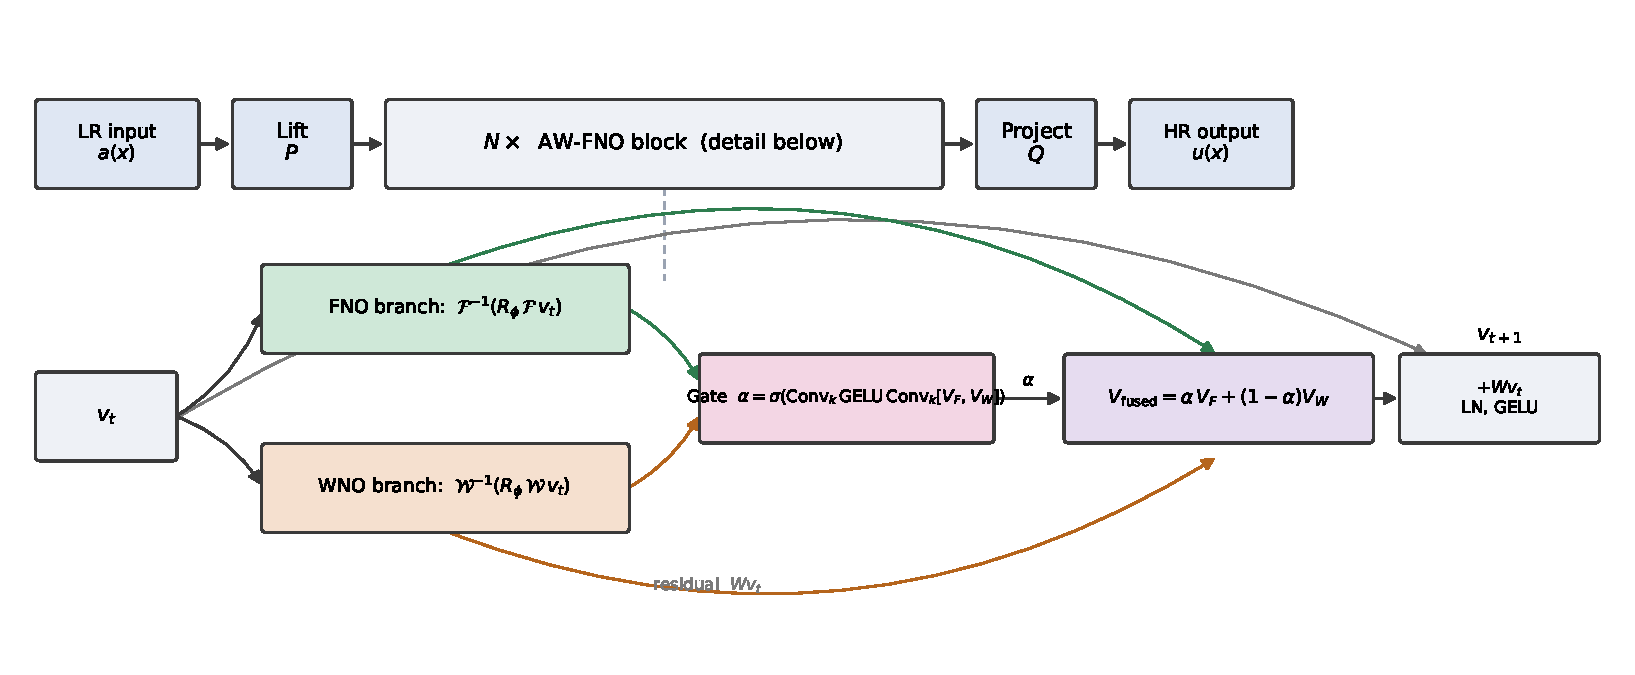
\includegraphics[width=1\linewidth]{figures/arch.pdf}
    \caption{Architecture of the Augmented Wavelet Fourier Neural Operator}
    \label{fig:awfno}
\end{figure}

\subsection{Mathematical Formulation}

The update for a hidden state $v_t$ to $v_{t+1}$ fuses the two branches through a spatially varying gate $\alpha(x)$:

\begin{equation}
    v_{t+1}(x) = \sigma \left( W v_t(x) + \alpha(x) \odot (\mathcal{K}_{F} v_t)(x) + \big(1 - \alpha(x)\big) \odot (\mathcal{K}_{W} v_t)(x) + b(x) \right),
    \laeq{update}
\end{equation}

where $\alpha(x) \in [0,1]$ is the adaptive gate produced by the gated fusion mechanism of Section~\ref{sec:gate}, $\odot$ denotes element-wise (channel-wise) multiplication, $x$ is input from the domain, $W$ is a local linear Operator %transformation%
%(residual connection)%
, $\mathcal{K}_{F}$ is the Fourier %integral%
kernel operator, defined as $(\mathcal{K}_{F}(\phi) \ast (v_t))(x)$ $=$ $\mathcal{F}^{-1}({R}_{\phi} \cdot \mathcal{F}(v_t))(x)$, where $\mathcal{F}$ is Fourier transform, $\mathcal{F}^{-1}$ is inverse Fourier transform, $R_\phi$ is a neural network-parameterized representation of the kernel $k$ in Fourier space with some parameter $\phi \in \mathcal{R}^{P}$.
$\mathcal{K}_{W}$ is the Wavelet kernel operator, defined as 
\begin{equation}
(\mathcal{K}_{W}(\phi) \ast (v_t))(x) = \mathcal{W}^{-1}({R}_{\phi} \cdot \mathcal{W}(v_t))(x)
\end{equation}
where $\mathcal{W}$ is wavelet transform, $\mathcal{W}^{-1}$ is inverse wavelet transform, and  $R_\phi$ is a neural network-parameterized representation of the kernel $k$ in wavelet space with
some parameter $\phi \in \mathcal{R}^{P}$. $b$ is a bias function and $\sigma$ is a non-linear activation function.

\subsection{Adaptive Spatial Gate}
\label{sec:gate}

% \textbf{Mechanism.} Adaptive Decisiveness via Entropic Regularization

% The AW-FNO utilises an entropy-regularised objective function to overcome the "mean-field" stagnation common in multi-stream neural operators. In standard gating implementations, gradient descent often settles into a suboptimal equilibrium where both the Fourier and Wavelet branches are under-utilised. We introduce a Shannon Entropy penalty on the latent spatial gate $\alpha(x)$. This regularizer acts as a structural bottleneck, pushing the probability distribution of the gating activations toward a Bernoulli-like state. Mathematically, this enforces a local expert regime: \\
% \textbf{Low-Entropy State.} The gate is forced to identify regions where the Fourier basis is numerically inefficient (e.g., near discontinuities) and switch entirely to the Wavelet basis.Resolution of Gibbs Phenomenon: By forcing the model to "turn off" the Fourier branch near shocks, we prevent the propagation of spectral ringing (Gibbs oscillations) into the final solution.

% \subsection*{Key Advantages for the Paper}
% \begin{itemize}
%     \item \textbf{Decoupling.} It prevents the Fourier and Wavelet layers from co-adapting to the same features, ensuring true multiresolution decomposition.
%     \item \textbf{Interpretability.} The resulting gate $\alpha(x)$ becomes a high-contrast map that identifies physical features (e.g., "The model used Wavelets here because there is a shock front").
%     \item \textbf{Stability.} In complex-valued fields, this prevents phase-instabilities by forcing the model to choose a single representation for local phase singularities.
% \end{itemize}

FNO and WNO learn complementary features. The FNO branch operates in the Fourier domain to capture global structures and long-range correlations, whereas the WNO branch uses localised wavelet representations, which excel at representing sharp gradients and multiscale local features. Consequently, no single operator is uniformly optimal across the entire spatial domain: smoothly varying regions and strongly discontinuous regions demand different representational strengths.

To exploit this complementary nature, we use the Adaptive Gated Fusion Mechanism (GFM) \cite{liu2025difffno} that performs spatially adaptive mixing of FNO and WNO features. Let 
\[
V_{\text{FNO}},\, V_{\text{WNO}} \in \mathbb{R}^{B \times H \times W \times C}
\]

represent the feature maps produced by FNO and WNO branches, respectively. We first concatenate these features along the channel dimension and pass them through a two-layer convolutional gate with kernel size $k=5$ and spatial padding, followed by a sigmoid activation, producing a per-channel gating map $\alpha \in \mathbb{R}^{B \times H \times W \times C}$ :
\[
\alpha = \sigma\Big(\mathrm{Conv}_{k}\big(\mathrm{GELU}\big(\mathrm{Conv}_{k}([V_{\text{FNO}},\, V_{\text{WNO}}])\big)\big)\Big).
\]
The kernel size is chosen so that the gate's effective receptive field (a $9$-pixel window for $k=5$ stacked twice) exceeds the characteristic width of the sharp features in the data --- approximately $5$--$10$ grid points for Burgers shocks at $\nu = 10^{-3}$. A single $1\times1$ convolution, having no spatial context, cannot express the spatial routing pattern and collapses to a near-uniform gate; the spatial receptive field is what enables the gate to localise sharp features.

The gate $\alpha$ at spatial location induces a piece-wise trust map that encodes the relative importance of FNO versus WNO. The fused representation is then obtained via an element-wise combination,

\[
V_{\text{fused}} = \alpha \odot V_{\text{FNO}} + (1 - \alpha) \odot V_{\text{WNO}},
\]

where the gating is applied element-wise per channel, allowing different feature channels to route independently. In regions where the underlying solution is smooth and globally coherent, the model learns \(\alpha \approx 1\), thereby prioritising the FNO branch and preserving large-scale consistency. Whereas, near the sharp interfaces, discontinuities or highly localised structures, the gate tends to shift to $0$, increasing the contribution of WNO and attenuating global spectral effects analogous to the Gibbs phenomenon that arise in purely Fourier-based representations. The GFM provides a router between the two experts, enabling data-dependent choice of expert while yielding a more robust and expressive hybrid operator.

\subsection{Entropy-Regularised Gating}
\label{sec:entropy}

Trained with a data-fidelity loss alone, the gate is prone to a ``mean-field'' stagnation in which it settles at the indecisive equilibrium $\alpha \approx \tfrac{1}{2}$ everywhere, so that both branches are averaged uniformly and the spatial routing of Section~\ref{sec:gate} never emerges. To break this symmetry, we add a Shannon-entropy penalty on the gate activations to the training objective,

\begin{equation}
    L_{\text{total}} = L_{\text{data}} + \lambda_{\text{ent}} \, \mathbb{E}_{x}\big[ H(\alpha(x)) \big],
    \qquad
    H(\alpha) = -\alpha \log \alpha - (1-\alpha)\log(1-\alpha),
    \laeq{entropy}
\end{equation}

with $\lambda_{\text{ent}} = 0.01$. The penalty drives the per-location gate towards a near-binary (Bernoulli) state, encouraging the model to commit to the locally more appropriate basis --- the Fourier branch in smooth, globally coherent regions and the wavelet branch near sharp gradients and discontinuities --- rather than averaging the two. Combined with a small random initialisation of the gate convolution (which displaces the gate from the exact $\alpha = \tfrac{1}{2}$ saddle point), this regulariser produces decisive, spatially varying routing.


% \subsection{Loss function}
% We use a loss function that ensures pixel-wise accuracy while also accounting for violations of the governing equation.

% \begin{equation*}
%     L = L_{MSE} + \lambda L_{Physics}.
% \end{equation*}


\section{Experiments}
\label{sec:experiments}

\subsection{Dataset}
\label{sec:dataset}

We evaluate AW-FNO on the spatial super-resolution of two-dimensional
forced Navier--Stokes turbulence. The data are vorticity snapshots
$\omega(x,y)$ of the forced incompressible Navier--Stokes equations on
the periodic torus $[0, 2\pi)^2$ at a viscosity corresponding to
Reynolds number $\mathrm{Re}\approx 10^{3}$, providing a turbulent
field rich in multi-scale coherent structures. The high-resolution (HR)
target is the $128 \times 128$ snapshot; the low-resolution (LR) input
is obtained by $4\times$ average-pooling to $32 \times 32$ followed by
bicubic upsampling back to $128 \times 128$, so the network learns the
LR$\rightarrow$HR residual on a fixed grid. We use $8{,}000$ snapshots
for training and $2{,}000$ for testing, with fields normalised to zero
mean and unit variance using statistics computed on the training set.

\subsection{Baselines and Ablation Variants}
\label{sec:baselines}

We compare AW-FNO against the following models, all trained under an
identical optimisation protocol (Section~\ref{sec:implementation}):

\begin{itemize}
  \item \textbf{Bicubic} --- the no-model baseline; the relative error
  of the bicubic-upsampled LR input itself, quantifying the difficulty
  of the task.
  \item \textbf{FNO} \cite{li2021fourier} --- a standard Fourier
  Neural Operator with $4$ layers, $32$ hidden channels and
  $20\times20$ retained Fourier modes.
  \item \textbf{FNO-fat} --- a parameter-augmented FNO with $128$
  hidden channels. This isolates whether additional spectral capacity
  alone closes the gap to AW-FNO, addressing the fairness of the
  comparison.
  \item \textbf{WNO} \cite{TRIPURA2023115783} --- a Wavelet Neural
  Operator branch ($4$ layers, $32$ channels, \texttt{db4} wavelet,
  decomposition level $3$).
\end{itemize}

To isolate the contribution of the adaptive gate, we evaluate three
ablations of AW-FNO that share the same dual-branch backbone (FNO
modes $20\times20$, WNO \texttt{db6} at level $3$, $32$ channels) and
differ only in the fusion mechanism:

\begin{itemize}
  \item \textbf{Fixed $\alpha=0.5$} --- the two branches are averaged
  with a constant, non-learnable weight, removing all spatial routing.
  \item \textbf{$1\times1$ gate} --- the gate is a single $1\times1$
  convolution followed by a sigmoid, i.e. a per-pixel channel mixing
  with \emph{no} spatial receptive field.
  \item \textbf{Rich gate} ($k=5$, $2$ layers) --- the proposed gate of
  Section~\ref{sec:gate}, with a $9\times9$ effective receptive field,
  trained with the entropy regulariser ($\lambda_{\text{ent}}=0.01$) and
  random gate initialisation.
\end{itemize}

\subsection{Evaluation Metrics}
\label{sec:metrics}

We report (i) the \emph{relative $L_2$ error}, our primary accuracy
metric; (ii) the \emph{relative $H_1$ error}, which is sensitive to the
accuracy of spatial gradients and hence to sharp features; (iii) the
\emph{high-frequency spectral $L_2$ error}, the relative error
restricted to wavenumbers above the LR Nyquist cutoff, which directly
measures recovery of the small-scale content that bicubic upsampling
discards and that Fourier methods tend to corrupt with Gibbs
oscillations; and (iv) the \emph{enstrophy error}
$|\mathcal{E}_{\text{pred}}-\mathcal{E}_{\text{true}}|/\mathcal{E}_{\text{true}}$
with $\mathcal{E}=\tfrac{1}{2}\!\int \omega^2\,dx$, a physically
meaningful diagnostic of the predicted vorticity field. To characterise
the gate we additionally report its mean Shannon entropy
$\mathbb{E}_x[H(\alpha)]$ (lower means more decisive routing) and the
Pearson correlation $\rho\big((1-\alpha),\,|\nabla\omega|\big)$ between
the WNO-routing weight and the vorticity-gradient magnitude of the
target (positive means the gate selects the wavelet branch at sharp
features).

\subsection{Implementation Details}
\label{sec:implementation}

All models are trained for $500$ epochs with the Adam optimiser
(learning rate $10^{-3}$, weight decay $10^{-4}$), a step-decay
schedule that halves the learning rate every $100$ epochs, gradient
clipping at $1.0$, and a batch size of $16$. Training minimises the
relative $L_2$ loss; for the rich-gate model the entropy penalty of
Eq.~\equa{entropy} is added with $\lambda_{\text{ent}}=0.01$. All runs
use a fixed random seed and are executed on a single $48$~GB NVIDIA
GPU. The checkpoint with the lowest test relative $L_2$ is retained for
evaluation.

\section{Results and Discussion}
\label{sec:results}

\subsection{Super-Resolution Accuracy}
\label{sec:results-main}

Table~\ref{tab:sr-main} reports the test-set performance of all models
on the $128^2$ super-resolution task. Every neural operator improves on
the bicubic baseline by more than an order of magnitude in relative
$L_2$ error (from $0.413$ down to $0.019$ for the plain operators and to
$0.0094$ for AW-FNO with the rich gate), confirming that the small-scale
content removed by $4\times$ downsampling is genuinely recoverable and
that the task is non-trivial.

% Auto-generated companion table: scripts/aggregate_sr_results.py writes
% outputs/tables/sr_main_table.{csv,tex}. Numbers below are transcribed
% from that CSV (best-epoch metrics).
\begin{table}[t]
  \centering
  \caption{Super-resolution results on forced Navier--Stokes $128^2$
  (best-epoch test metrics; lower is better for all columns except where
  noted). High-$f$ $L_2$ is the relative spectral error above the LR
  Nyquist cutoff. Gate entropy $H$ is reported only for gated variants.}
  \label{tab:sr-main}
  \begin{tabular}{lcccccc}
    \hline
    Model & Params & Rel $L_2$ & Rel $H_1$ & High-$f$ $L_2$ & Enstrophy & Gate $H$ \\
    \hline
    Bicubic (no model)            & ---    & 0.4134 & ---    & ---    & ---     & ---    \\
    FNO                           & 0.91M  & 0.0193 & 0.152  & 303.8  & 6.2e-4  & ---    \\
    FNO-fat ($c{=}128$)           & 14.6M  & 0.0198 & 0.157  & 325.3  & 5.6e-4  & ---    \\
    WNO                           & 81.6M  & 0.0179 & 0.159  & 180.6  & 9.8e-4  & ---    \\
    AW-FNO (fixed $\alpha{=}0.5$) & 89.3M  & 0.0210 & 0.194  & 265.7  & 1.3e-3  & ---    \\
    AW-FNO ($1{\times}1$ gate)    & 89.3M  & 0.0134 & 0.116  & 173.7  & 1.4e-3  & 0.667  \\
    \textbf{AW-FNO (rich gate)}   & 89.3M  & \textbf{0.0094}$^\dagger$ & \textbf{0.083} & \textbf{113.0} & 7.4e-4 & \textbf{0.017} \\
    \hline
    \multicolumn{7}{l}{\footnotesize $^\dagger$Rich-gate run still completing (epoch 317/500, error still decreasing); value provisional.}\\
  \end{tabular}
\end{table}

Several findings emerge. \emph{(i)} Among single operators the wavelet
branch is strongest on the small scales: the WNO attains the lowest
high-frequency spectral error ($180.6$ versus $303.8$ for the FNO),
consistent with its multi-resolution basis being better suited to
localised vorticity gradients and with the Gibbs-suppression argument of
Section~\ref{sec:gate}. \emph{(ii)} Additional Fourier capacity alone
does not help: the parameter-augmented FNO-fat ($14.6$M parameters) is
statistically indistinguishable from the standard FNO ($0.0198$ versus
$0.0193$), confirming that the gains below come from the dual-branch
fusion rather than from raw model size. \emph{(iii)} The fusion must be
\emph{learned}: a non-adaptive average of the two branches
($\alpha=0.5$) is in fact worse than either branch alone ($0.0210$),
whereas making the mixing coefficient learnable --- even with a
spatially-blind $1\times1$ gate --- lowers the error to $0.0134$, below
both single operators. \emph{(iv)} Accuracy and interpretability are,
however, distinct: the $1\times1$ gate's entropy stays near the
indecisive value ($H\approx0.67$, cf.\ $\ln2\approx0.693$) and its
routing is spatially flat (Section~\ref{sec:results-gate}), so its gain
stems from a learned per-channel re-weighting rather than from
feature-aware spatial routing. Endowing the gate with a spatial
receptive field (the rich gate) delivers both: it attains the best
accuracy on every error metric (relative $L_2 \approx 0.0094$, a
$\sim$48\% reduction over the best single operator and $\sim$30\% over
the $1\times1$ gate) \emph{and} a decisive, spatially structured gate
($H\approx0.017$), which we examine in
Sections~\ref{sec:results-spectrum}--\ref{sec:results-gate}.

% TODO: rich-gate run still completing (ep~325/500) — refresh the exact
% rich-gate digits in the table + this paragraph from
% scripts/aggregate_sr_results.py once it hits epoch 500.

\subsection{Energy Spectrum}
\label{sec:results-spectrum}

To assess the physical fidelity of the reconstructed fields beyond
point-wise error, we compute the radially averaged kinetic-energy
spectrum $E(k)$ and compare each model against the ground-truth HR
field (Figure~\ref{fig:spectrum}, generated by
\texttt{scripts/energy\_spectrum\_sr.py}). The bicubic baseline collapses
above the LR Nyquist wavenumber, having no energy to place there. The
key diagnostic is the high-$k$ inertial range: an operator that
over-smooths loses energy there, while one that produces Gibbs ringing
overshoots it. % TODO: insert the measured E(k) comparison once the
% rich-gate run completes and the figure is regenerated.

\subsection{Gate Routing Analysis}
\label{sec:results-gate}

The central architectural claim of this work is that a
spatially-resolved gate learns to route the wavelet branch to sharp
features and the Fourier branch to smooth regions. We test this on the
trained rich-gate model by extracting the per-block gate maps
$\alpha(x,y)$ and correlating the WNO-routing weight $(1-\alpha)$ with
the vorticity-gradient magnitude $|\nabla\omega|$ of the target
(Figure~\ref{fig:gatemap}, produced by
\texttt{scripts/analyze\_gate\_sr.py}). A positive correlation
$\rho\big((1-\alpha),|\nabla\omega|\big)$ is direct evidence of the
claimed routing behaviour.

As a negative control, the $1\times1$-gate variant produces an almost
spatially constant gate: across the deepest fusion block its map has
mean $\bar\alpha\approx0.52$ but a spatial standard deviation of only
$\approx10^{-3}$, and a routing correlation of merely
$\rho\approx+0.03$. The gate therefore carries essentially no spatial
information and reduces to a near-uniform average of the two branches,
consistent with its collapsed entropy ($H\approx0.68$,
Table~\ref{tab:sr-main}) and with the Phase-2 finding on the Burgers
equation. This confirms that a spatial receptive field --- not merely a
learnable mixing coefficient --- is what enables feature-aware routing.

% TODO: report the measured rho and discuss
% whether the Phase-2.5 Burgers result (rho up to +0.32) transfers to
% the 2D turbulence regime, framing the outcome as regime
% characterization (adaptive routing helps on spatially heterogeneous
% fields; uniform mixing suffices on statistically homogeneous ones).


\section{Conclusions}

This work proposes AW-FNO, an adaptive hybrid neural operator that combines the complementary strengths of Fourier and Wavelet representations for fluid flow super-resolution. With the integration of a parallel architecture with an adaptive gated fusion mechanism, we are able to capture the localised multiscale features. The entropy-regularised gating strategy promotes decisive, spatially varying selection between the two operators, thereby enhancing robustness near sharp gradients and discontinuities, and reducing spectral artefacts, such as Gibbs oscillations.

\textbf{The AW-FNO introduces a hybrid neural operator framework that synergistically integrates the global spectral efficiency of FNOs with the multi-resolution localisation of WNOs for super-resolving turbulent flows. The fusion of parallel kernel architecture and adaptive GFM enables spatially varying feature selection. The model learns to prioritise FNO for smooth, large-scale coherent structures and WNO for sharp gradients, discontinuities and small-scale eddies. This routing behaviour requires the gate to have sufficient representational capacity: a single $1\times1$ convolution cannot express the spatial routing pattern, whereas a gate with a spatial receptive field can. This architectural design overcomes FNO's limitations such as Gibbs oscillations and spectral bias near local discontinuities, resulting in high fidelity reconstruction, enhanced generalisation across unseen resolutions and reduced computational overhead compared to traditional DNS or standalone NOs.}

\textbf{Experiments demonstrate AW-FNO's robustness on high-Reynolds turbulent benchmarks, achieving zero-shot super-resolution. Future extensions could be dealing with 3D unstructured meshes via graph integrations, further bridging the gap toward real-time CFD surrogates.}






%%%% BIBLIOGRAPHY
\bibspacing=\dimen 10
\bibliographystyle{unsrt} 
\bibliography{biblio}


\end{document}

% Some suggestions (Harshdeep Sharma): 

% Introduction should contain some references about what problem you are going to solve and why it matters. 
% Secondly, you should try to show that the problem falls in the literature as a gap. 
% Then, from a higher level, i see that you can move that 'The core .. flucutations' para in the Introduction itself. 
% Also, Section 2 should start with Mathematical formulation and then section 3 or 2(b) can include the architecture or the numerical implementation details. 
% Then currently, 'Key Advantages.. singularities' can be moved to the introduction or in conculsions. 
% Before, Conclusions there will be a section on Results and Discussions. 